\documentclass{beamer}

\usepackage[utf8]{inputenc}
\usepackage{default}
\usepackage{pslatex}
\usepackage{graphicx}
\usepackage{algorithmic}
\usepackage{multicol}

\renewcommand{\algorithmicfor}{\textbf{Pour}}
\renewcommand{\algorithmicendfor}{\textbf{Fin Pour}}
\renewcommand{\algorithmicdo}{\textbf{Faire}}
\renewcommand{\algorithmicif}{\textbf{Si}}
\renewcommand{\algorithmicendif}{\textbf{Fin Si}}
\renewcommand{\algorithmicthen}{\textbf{Alors}}
\renewcommand{\algorithmicreturn}{\textbf{Retourner}}

\usetheme{Warsaw}

\title{Comment simuler numériquement l'évolution de la géomorphologie alpines ?}
\subtitle{Sujet de TPE}
\author{Gros Alexis, Manceau Thibaut, Porteries Tristan}
\logo{
\includegraphics[height=0.5cm]{blender.png}}

\makeindex

\useoutertheme{infolines}

\begin{document}

% Titre
\frame{\titlepage}

% Sommaire
\begin{frame}{Sommaire}
\small \tableofcontents
\end{frame}

\section{Déroulement du projet sur SysMl}
\begin{frame}
   \begin{center}
      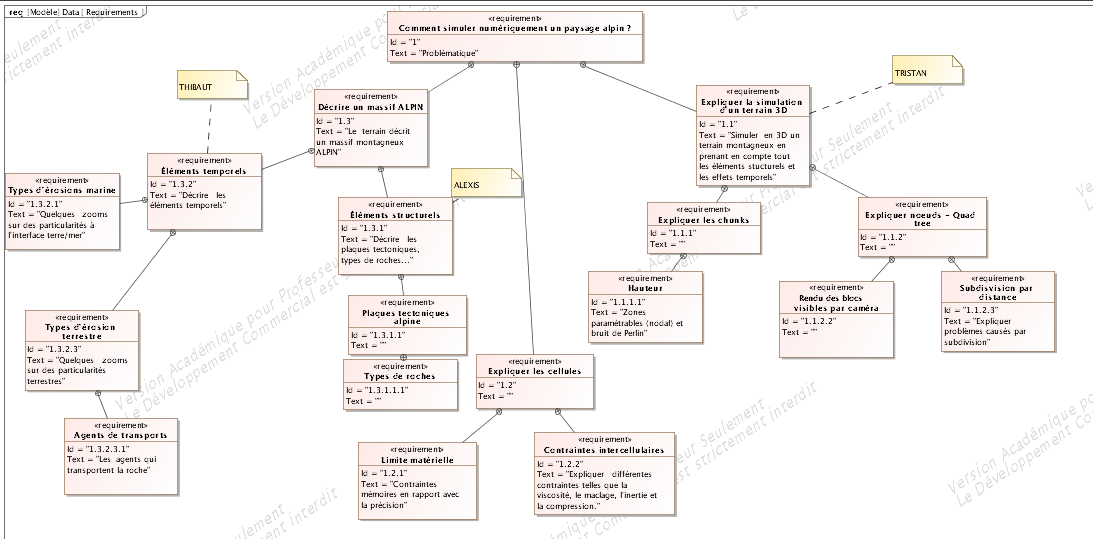
\includegraphics[width=8cm]{sysml.png}
   \end{center}
   Pour organiser le déroulement du projet nous avons réalisé un diagramme avec SysMl.
\end{frame}

\section{Les chunks}
\begin{frame}
  Définition : Ce sont des morceaux de terrain carrés composés du même nombre de vertices formant une grille déformée en profondeur (Z).
  Tous ces vertices forment des triangles.
  \begin{center}
    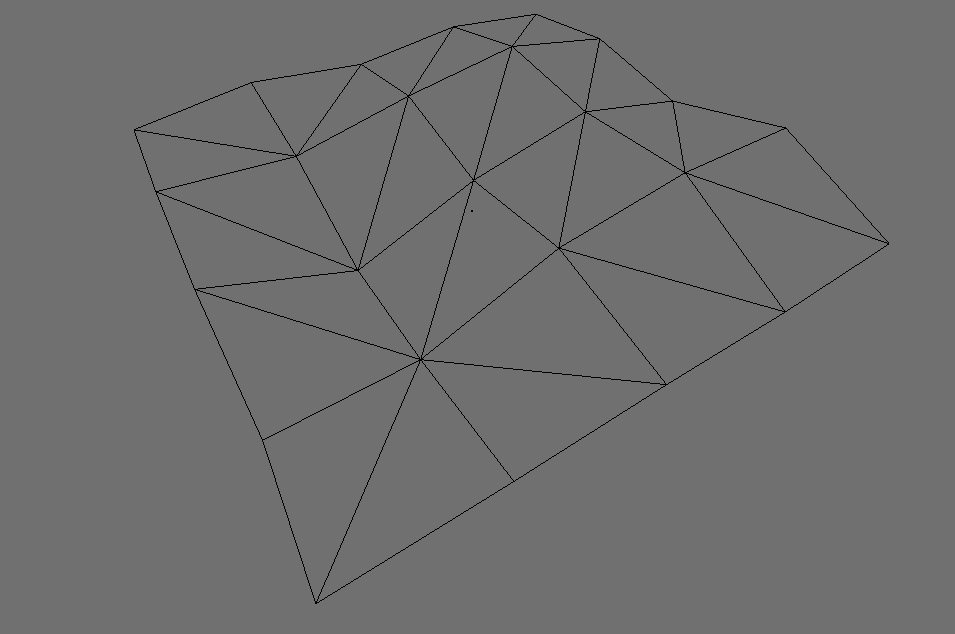
\includegraphics[width=8cm]{chunk_simple_wireframe.png}
  \end{center}
\end{frame}

\section{Les arbres binaires à 2 dimensions (QuadTree)}
\begin{frame}
  C'est un arbre à 2 dimensions qui pour chaque noeud (carré 2D) contient 4 sous noeuds 2 fois plus petit.
  Chaque fonction d'un noeud peut être appliquée à ses sous noeuds.
  \begin{center}
    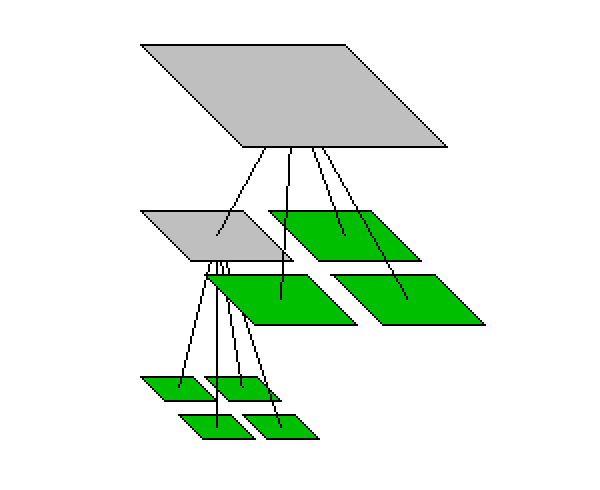
\includegraphics[width=4cm]{picture_quadtree.png}
    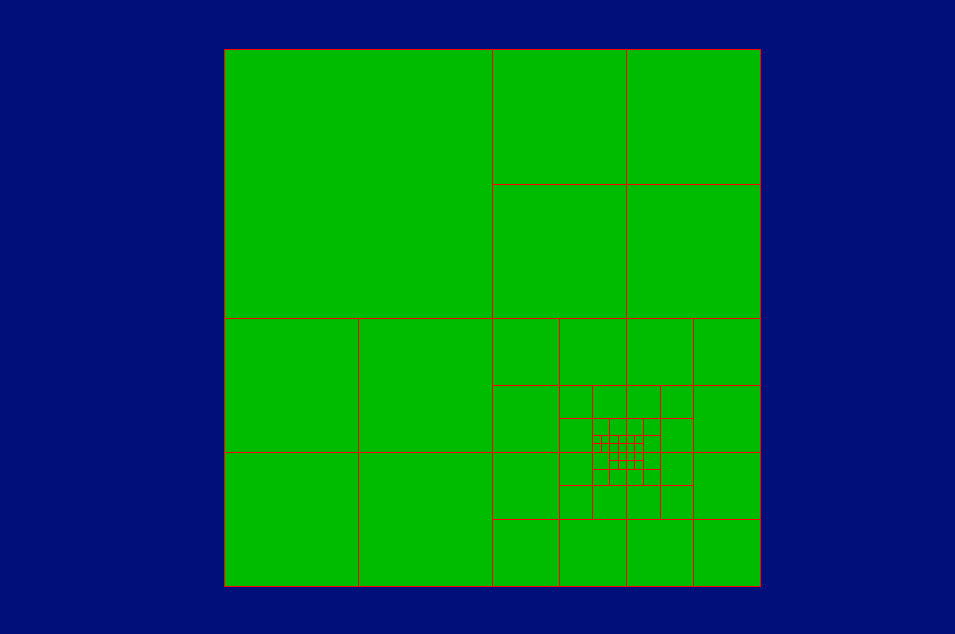
\includegraphics[width=6cm]{terrain_quadtree.png}
  \end{center}
\end{frame}

\section{La subdivision des noeuds}
\begin{frame}
  Chaque noeud est subdivisé en fonction de la distance du bord le plus proche de ce noeud vers la caméra.
  \begin{algorithmic}[1]
    \STATE $d = \max(\left\|\overrightarrow{CN}\right\| - r, 0)$
    \FOR{$n$ de $0$ jusqu'à $(n_{max} - 1)$}
      \IF{$\frac{d_{max} \times n}{n_{max}} <= d < \frac{d_{max} \times (n + 1)}{n_{max}}$}
	\RETURN $n_{max} - n$
      \ENDIF
    \ENDFOR
  \end{algorithmic}
  $n_{max}$ : niveau de subdivisions maximale, $C$ : position de la caméra, $N$ : centre du noeud, 
  $d_{max}$ : distance maximale pour subdiviser un noeud, $r$ : rayon du noeud.
\end{frame}

\section{La Visibilité des noeuds dans le champ de vue (Frustum Culling)}
\begin{frame}
    Pour savoir si un noeud est visible on teste si sa boîte englobante alignée (AABB) est dans le champ de la caméra.
    \begin{center}
      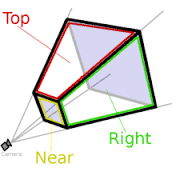
\includegraphics[width=2cm]{frustum_culling_cone.png}
    \end{center}
    \begin{center}
      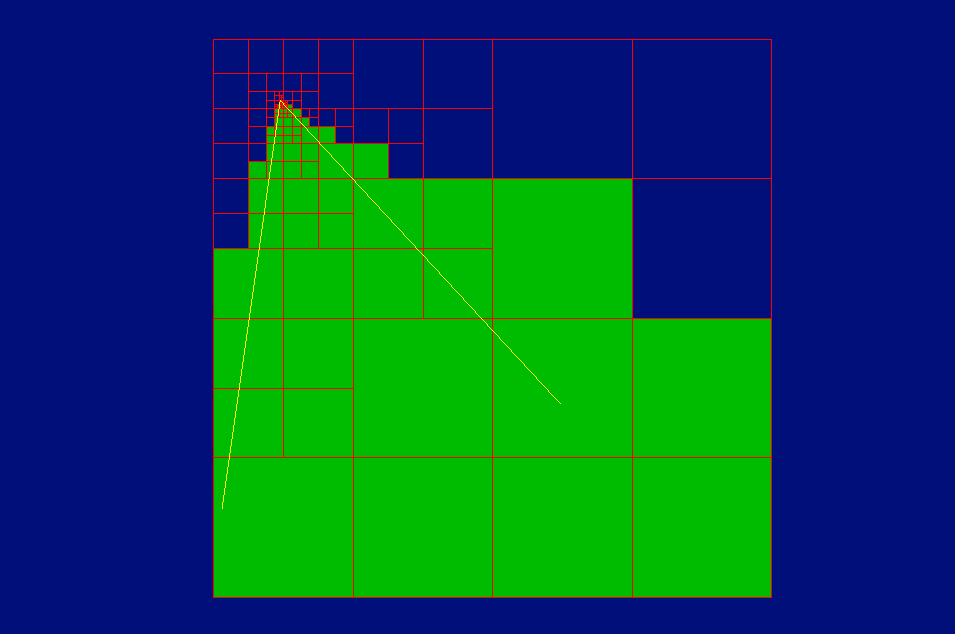
\includegraphics[width=5cm]{terrain_culling_0.png}
      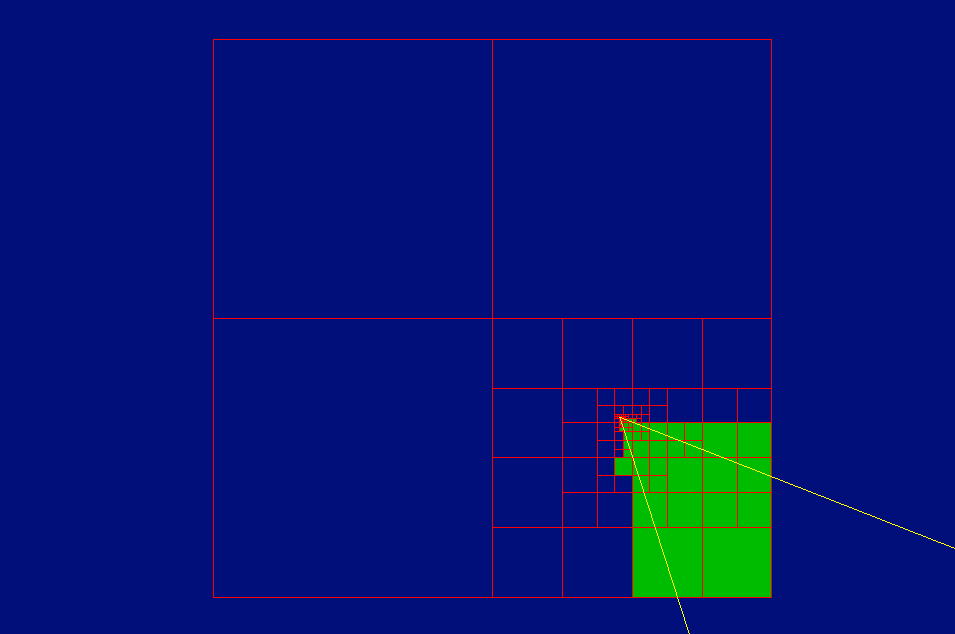
\includegraphics[width=5cm]{terrain_culling_1.png}
    \end{center}   
\end{frame}

\begin{frame}
  \begin{multicols}{2}
    \begin{algorithmic}[1]
      \STATE $c_1 = 0$
      \FOR{$p$ de $1$ jusqu'à $6$}
	\STATE $c_2 = 0$
	\FOR{$v$ de $1$ jusqu'à $8$}
	  \IF{$\overrightarrow{P_p} \ldotp \overrightarrow{B_v} < 0$}
	    \STATE $c_2 = c_2 + 1$
	  \ENDIF
	\ENDFOR
	\IF{$c_2 = 8$}
	  \RETURN Dehors
	\ELSE
	  \STATE $c_1 = c_1 + 1$
	\ENDIF
      \ENDFOR
      \IF{$c_1 > 0$}
	\RETURN Intersection
      \ELSE
	\RETURN Interieur
      \ENDIF
    \end{algorithmic}
  \end{multicols}
  $P_n$ : matrice $4 \times 3$ du plan $n$ de la caméra, $B_n$ : la position du coin $n$ de la boîte de visibilité.
\end{frame}

\end{document}
